\subsection{Properties of the LCA}
\label{sec:meta}

When merging two concurrent versions $v_1$ and $v_2$, the common
ancestor argument for \C{merge} must be the LCA of $v_1$ and $v_2$,
without which \C{merge} may yield unexpected results. This is
demonstrated for the grow-only counter in
Fig.~\ref{fig:merge-needs-lca}, where an incorrect count is obtained if a
common ancestor that is not an LCA is used to merge 4 and 7. While in
this example there is a unique LCA for 4 and 7, in general this may
not be the case. With unrestrained branching and merging, there is no
bound on the number of LCAs a pair of versions can have.  For example,
in Fig.~\ref{fig:criss-cross-lcas}, the merge of 0 with 3 is preceded
by two ``criss-cross'' merges between their respective branches
resulting in there being two LCAs (5 and 4) for 0 and 3.
% Multiple LCAs can occur even without criss-cross merges, as
% demonstrated by Fig.~\ref{fig:external-lcas}.
Concurrent versions with multiple LCAs do not lend themselves to
three-way merging. If such versions represent the tips of their respective
branches, they render the branches unmergeable (since  \C{lca} is no
longer a function). This problem also arises in the context of source
control systems, which employ \emph{ad hoc} mechanisms to pave the way
for three-way merging.  GitHub~\cite{github}, for instance,
recursively merges LCAs to compute a virtual ancestor, which then
\begin{wrapfigure}{L}{.4\textwidth}
\centering
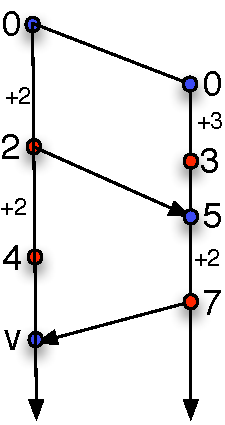
\includegraphics[scale=0.45]{Figures/merge-needs-lca}
\caption{This example of a grow-only counter illustrate why \C{merge}
needs a least common ancestor, and not just a common ancestor. Both 0
and 2 are common ancestors of 4 and 7, while 2 is their least common
ancestor (since $0 \preceq 2$). The result (v) of merging 4 and 7 is
11 (incorrect) if 0 is used as the common ancestor for merge, and 9
(correct, because 2+2+3+2 = 9) if 2 is used. }
\label{fig:merge-needs-lca}
\end{wrapfigure}
serves as the LCA for merging concurrent versions. This method is
demonstrated in the branching structure for a mergeable, replicated
counter as shown in Fig.~\ref{fig:criss-cross-lcas}, where LCAs 5 and
4 of 0 and 3 are merged (with their LCA being 10) to generate -1 as
the virtual LCA to merge 5 and 4. A major downside with this approach
is that it makes no guarantees on the relationship between the virtual
ancestor and its concurrent versions; the former may not even be a
legal ancestor of the latter as per the semantics of the data type.
For instance, suppose the integer type in
Fig.~\ref{fig:criss-cross-lcas} represents a bank account balance,
which is expected to disallows any activity on the account if the
balance is ever known to be less than zero.  From the perspective of
the library designer and its clients, there is no meaningful scenario
in which versions 3 and 0 can emerge from -1, since the only
transition allowed by the semantics from -1 is to itself.  Clearly,
\emph{ad hoc} mechanisms like this are error-prone and difficult to
apply in general.

\begin{figure}[!t]
\centering
\subcaptionbox[] {\small
  In this example, 1 and 3 have two LCAs (3 and 4) a result of
  previous merges. The dotted circle denotes a virtual ancestor
  obtained by merging the two LCAs.
  \label{fig:criss-cross-lcas}
} [0.47\columnwidth] {
  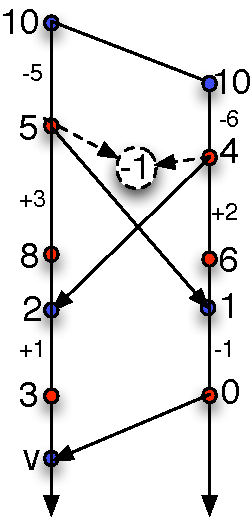
\includegraphics[scale=0.55]{Figures/2-LCAs}
}
% \hfill
% \subcaptionbox[] {\small
%   In this example, versions $v_{13}$ and $v_{44}$ have two LCAs
%   ($v_{22}$ and $v_{32}$)  despite there not being any previous merges
%   between their respective branches.
%   \label{fig:external-lcas}
% } [0.47\columnwidth] {
%   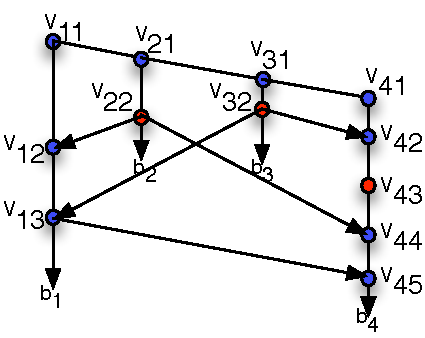
\includegraphics[scale=0.7]{Figures/2-external-LCAs}
% }
\caption{Examples where merging versions have more than one LCA}
\label{fig:many-lcas}
\end{figure}

Fortunately, unlike source control systems where branching structure
is entirely dictated by the user, \name abstracts away branching
structure from the programmer, and hence retains the ability to
manifest it in a way that it deems fit. In particular, \name solves
the problem of criss-cross merges by constraining the branching
stucture to prevent their existence. As captured in the operational
semantics, this is done by restricting the merge operation only to the
tips (latest versions) of the branches. For instance, suppose $v_{11}$
and $v_{21}$ are the latest versions on branches $b_1$ and $b_2$,
respectively. Merging $b_2$ into $b_1$ entails merging $v_{21}$ into
$v_{11}$ to generate version $v_{12}$ on $b_1$.  Now, merging $b_1$
into $b_2$ involves merging $v_{12}$, the latest version on $b_1$,
into $v_{21}$, but not $v_{11}$ into $v_{21}$, thus preempting a
criss-cross branching structure.
% In other words, a criss-cross branching structure is prevented due
% to the order among merges between conflicting branches introduced as
% a result of \rulelabel{E-Pull-Wait} being an atomic step.

% Next, for branching structures where a pair of branches (i.e., their
% respective latest versions) have multiple externally-located LCAs, we
% suitably extend the branching structure to generate a new single LCA.
%  For instance, consider
% the example in Fig.~\ref{fig:external-lcas}, where (latest versions
% on) branches $b_1$ and $b_4$ have two externally-located LCAs
% ($v_{22}$ and $v_{32}$), hence cannot be merged. Mergeability can
% however be reclaimed by extending the branching structure as shown in
% Fig.~\ref{fig:legal-extension-1}. The extension is done by first
% merging $b_3$ into $b_2$ to create version $v_{23}$ on $b_2$, then
% merging $b_2$ into $b_1$ to create version $v_{14}$ on $b_1$, and
% finally merging $b_2$ into $b_4$ to create version $v_{45}$ on
% $b_4$. Observe that $b_1$ and $b_4$ now have a single LCA ($v_{23}$)
% hence are now mergeable. Mergeability could also have been reclaimed
% by adopting an alternative extension to the branching structure as
% shown in Fig.~\ref{fig:legal-extension-2}.

\begin{figure}[!t]
\centering
\subcaptionbox[] {\small
  In this example, versions $v_{13}$ and $v_{44}$ have two LCAs
  ($v_{22}$ and $v_{32}$) rendering their respective branches
  unmergeable.
  \label{fig:external-lcas}
} [0.47\columnwidth] {
  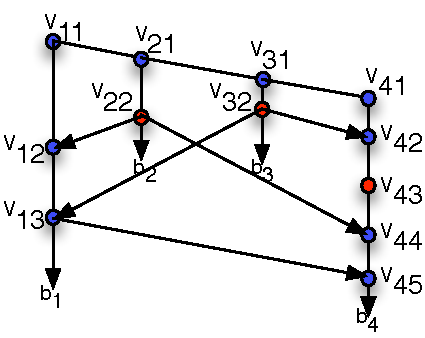
\includegraphics[scale=0.7]{Figures/2-external-LCAs}
}
\hfill
\subcaptionbox[] {\small
  However, execution can still progress to the depicted state, where
  $b_1$ and $b_4$ are again mergeable.
  \label{fig:legal-extension-1}
} [0.47\columnwidth] {
  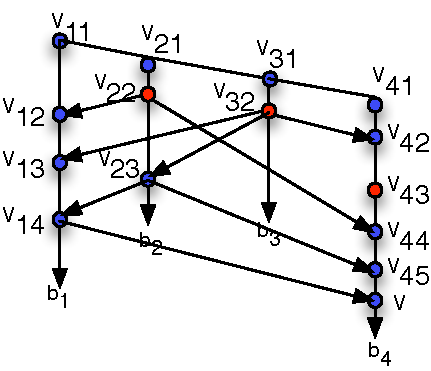
\includegraphics[scale=0.8]{Figures/legal-extension-1}
}
% \hfill
% \subcaptionbox[] {\small
%   $b_2$ is merged into $b_3$ to create $v_{33}$ here.
%   \label{fig:legal-extension-2}
% } [0.47\columnwidth] {
%   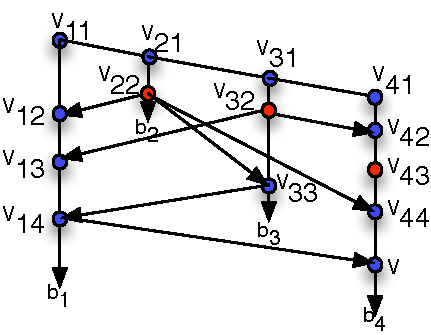
\includegraphics[scale=0.8]{Figures/legal-extension-2}
% }
\caption{Multiple LCAs without criss-cross merges do not threaten
the progress guarantee.}
\label{fig:legal-extensions}
\end{figure}

There can be other scenarios that lead to multiple LCAs, such as the
one shown in Fig.~\ref{fig:external-lcas}. However, preemption of
criss-cross merges is sufficient to make progress despite multiple
LCAs. For instance, the branching history in
Fig.~\ref{fig:external-lcas}, where $b_1$ and $b_4$ cannot merge due
to multiple LCAs, can still make progress to the history shown in
~\ref{fig:legal-extension-1}, where $b_1$ and $b_4$ are now mergeable.
We formalize the progress guarantee in the following theorem, whose
proof is included in the appendix.

\begin{theorem} [\bfseries Progress]
In a legal branching history $H$ produced by the operational
semantics, there exist at least two branches that have a unique LCA,
hence mergeable.
\end{theorem}
